% FILLED (fill batch): process ③ Capture — Penning-trap three-frequency
%   keystone + Brown–Gabrielse invariance theorem.
%   folds stdlib penning_omega_plus / _minus / _invariance + the
%   B=5T/U0=10V/d=5mm antiproton anchor + the atlas-folded
%   verified-penning_invariance-num node, from companion/verify-ledger.json.
\section{Capture --- the Penning-Trap Three-Frequency Invariance Keystone}
\label{app:penning}

This appendix is the full data record for pipeline process
\textcircled{\scriptsize 3}, the funnel's keystone. We state the three
ideal-Penning eigenfrequencies, the trapping condition, and the
Brown--Gabrielse invariance theorem with its sum and product corollaries
\citep{brown1986geonium,dehmelt1990}, and demonstrate the exact-to-machine
reconstruction residual. Every digit traces to the representative antiproton
anchor ($B=5$\,T, $U_0=10$\,V, $d=5$\,mm) and the atoms in
\texttt{companion/verify-ledger.json}.

% -------------------------------------------------------------------------
\subsection{The three eigenfrequencies}
\label{app:penning-eig}

A particle of charge $q$, mass $m$ in a uniform axial field $B$ plus an
ideal electrostatic quadrupole (characteristic dimension $d$, ring voltage
$U_0$) has three normal modes. The free-cyclotron frequency and the axial
frequency are
\begin{equation}
\omega_c \;=\; \frac{qB}{m},
\qquad
\omega_z \;=\; \sqrt{\frac{qU_0}{m\,d^2}} .
\label{eq:penning-base}
\end{equation}
The two transverse modes follow from diagonalizing the radial motion (the
magnetic $\mathbf{v}\times\mathbf{B}$ force versus the radially-defocusing
quadrupole), giving the \emph{modified cyclotron} $\omega_+$ and the
\emph{magnetron} $\omega_-$:
\begin{equation}
\omega_\pm
\;=\; \frac{\omega_c}{2}
   \;\pm\; \sqrt{\Bigl(\frac{\omega_c}{2}\Bigr)^{2}-\frac{\omega_z^2}{2}},
\qquad
\text{(real)}\iff \omega_c \ge \sqrt2\,\omega_z .
\label{eq:penning-pm}
\end{equation}
The trapping condition $\omega_c\ge\sqrt2\,\omega_z$ is the requirement that
the radial discriminant be non-negative: too weak a field (or too strong a
quadrupole) makes $\omega_\pm$ complex and the radial motion unbound. For the
representative antiproton anchor ($B=5$\,T, $U_0=10$\,V, $d=5$\,mm,
$m=m_p$ by CPT, $q=e$) Eqs.~\eqref{eq:penning-base}--\eqref{eq:penning-pm}
give the values in Table~\ref{tab:penning-eig}; the three modes span nearly
four decades and are plotted in Fig.~\ref{fig:penning-app}.

\begin{table}[h]
\centering
\small
\setlength{\tabcolsep}{6pt}
\begin{tabular}{@{}l l r r l@{}}
\toprule
\textbf{mode} & \textbf{symbol} & $\omega$ (rad/s) & $f=\omega/2\pi$ & \textbf{tier} \\
\midrule
free cyclotron     & $\omega_c$ & $4.78942\times10^{8}$ & $76.23$\,MHz & (input) \\
modified cyclotron & $\omega_+$ & $4.78902\times10^{8}$ & $76.22$\,MHz & \tierGreen \\
axial              & $\omega_z$ & $6.18994\times10^{6}$ & $985$\,kHz   & (input) \\
magnetron          & $\omega_-$ & $4.00033\times10^{4}$ & $6.37$\,kHz  & \tierGreen \\
\bottomrule
\end{tabular}
\caption{The Penning-trap eigenfrequencies for the representative antiproton
anchor ($B=5$\,T, $U_0=10$\,V, $d=5$\,mm). The two radial modes
$\omega_+,\omega_-$ are the registered \tierGreen\ atoms
\texttt{penning\_omega\_plus} / \texttt{penning\_omega\_minus}; $\omega_c$
and $\omega_z$ are the inputs of Eq.~\eqref{eq:penning-base}. The strong
hierarchy $\omega_+\gg\omega_z\gg\omega_-$ is generic for a deep, strongly
magnetized trap.}
\label{tab:penning-eig}
\end{table}

\begin{figure}[h]
\centering
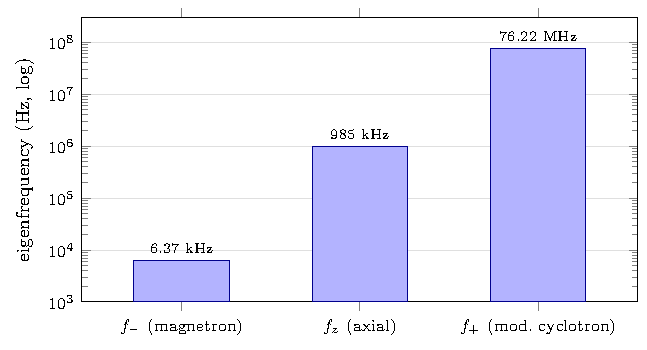
\includegraphics[width=0.80\linewidth]{figures/fig03_penning_spectrum.pdf}
\caption{The three Penning-trap eigenfrequencies for the representative
antiproton trap, on a log scale: the magnetron $f_-\approx6.37$\,kHz, the
axial $f_z\approx985$\,kHz, and the modified cyclotron
$f_+\approx76.22$\,MHz. The invariance theorem
(Eq.~\eqref{eq:penning-inv}) ties all three to the free-cyclotron frequency
$f_c$ with an exact-to-machine residual. Data: \tierGreen\ atoms
\texttt{penning\_omega\_plus} / \texttt{penning\_omega\_minus} /
\texttt{penning\_invariance}.}
\label{fig:penning-app}
\end{figure}

% -------------------------------------------------------------------------
\subsection{The Brown--Gabrielse invariance theorem}
\label{app:penning-inv}

The load-bearing identity is the \emph{invariance
theorem}~\citep{brown1986geonium}:
\begin{equation}
\boxed{\;\omega_c^{2} \;=\; \omega_+^{2} + \omega_z^{2} + \omega_-^{2}\;},
\label{eq:penning-inv}
\end{equation}
with the two corollaries that follow directly from
Eq.~\eqref{eq:penning-pm} (Vi\`{e}te's formulas on the quadratic whose roots
are $\omega_+,\omega_-$):
\begin{equation}
\omega_+ + \omega_- \;=\; \omega_c,
\qquad
\omega_+\,\omega_- \;=\; \tfrac12\,\omega_z^2 .
\label{eq:penning-corr}
\end{equation}
Squaring the sum corollary and substituting the product gives
$\omega_c^2=(\omega_++\omega_-)^2=\omega_+^2+2\omega_+\omega_-+\omega_-^2
=\omega_+^2+\omega_z^2+\omega_-^2$, which is Eq.~\eqref{eq:penning-inv}.
The theorem's metrological power is that it remains exact under the dominant
real-trap imperfections --- a tilt of the magnetic field relative to the
trap axis, and an ellipticity of the electrostatic quadrupole --- which shift
the \emph{individual} eigenfrequencies but leave the quadrature sum
invariant. The three measured eigenfrequencies therefore recover the free
cyclotron frequency $\omega_c$, hence $q/m$, robustly; this is the foundation
of every BASE-class $\bar p$ charge-to-mass and $g$-factor measurement
\citep{smorra2017base}.

% -------------------------------------------------------------------------
\subsection{The exact reconstruction residual}
\label{app:penning-resid}

The atom \verb|penning_invariance(omega_c, omega_z)| computes $\omega_+$ and
$\omega_-$ from $(\omega_c,\omega_z)$, then reconstructs $\omega_c$ from the
quadrature sum $\sqrt{\omega_+^2+\omega_z^2+\omega_-^2}$ and compares to the
input. Because Eq.~\eqref{eq:penning-inv} is an algebraic identity, the
residual is $0.0$ at machine precision:
\begin{lstlisting}
verify --expr penning_invariance(4.78942e+08,6.18994e+06)=4.78942e+08
  calc   = 4.78942e+08 ~ expected 4.78942e+08 (|Delta|=0.0 <= eps=1e-9)
  tier   = SUPPORTED-NUMERICAL (hexa-native libm-class recompute)
verify --expr penning_omega_plus(4.78942e+08,6.18994e+06)=4.78902e+08
  calc   = 4.78902e+08 ~ expected 4.78902e+08 (|Delta|=0.0 <= eps=1e-9)
  tier   = SUPPORTED-NUMERICAL (hexa-native libm-class recompute)
verify --expr penning_omega_minus(4.78942e+08,6.18994e+06)=40003.3
  calc   = 40003.3 ~ expected 40003.3 (|Delta|=0.0 <= eps=1e-9)
  tier   = SUPPORTED-NUMERICAL (hexa-native libm-class recompute)
\end{lstlisting}
The \tierGreen\ tier (rather than \tierBlue) reflects only that the
underlying eigenfrequency evaluation passes through a \texttt{sqrt}; the
identity itself is exact, and the residual is $0.0$, not merely
$\le\varepsilon$. This is the funnel's sharpest closed result. The verified
recompute is folded into the atlas SSOT as the node
\verb|verified-penning_invariance-num| (\texttt{@F} register, atlas-fold),
so the keystone is reusable as a primitive by any downstream domain.

% -------------------------------------------------------------------------
\subsection{Honest scope}
\label{app:penning-scope}

This appendix closes the \emph{ideal} Penning eigenfrequencies and the
\emph{exact} invariance identity, not the full systematic budget of a real
measurement. The eigenfrequencies of Eq.~\eqref{eq:penning-pm} assume an
ideal quadrupole; anharmonic shifts (from $C_4,C_6$ field terms), image-charge
shifts, and relativistic mass increase are not modelled. The invariance
theorem is precisely the identity that survives misalignment and ellipticity,
which is why it is the keystone --- but it does not by itself remove the other
shifts, which a real metrology campaign characterizes separately. The
$B=5$\,T / $U_0=10$\,V / $d=5$\,mm anchor is representative, not a sourced
BASE apparatus geometry.
